\documentclass[a4paper]{article}
\usepackage[utf8x]{inputenc}
\usepackage[T1,T2A]{fontenc}
\usepackage[russian]{babel}
\usepackage{hyperref}
\usepackage{indentfirst}
\usepackage{listings}
\usepackage{color}
\usepackage{here}
\usepackage{array}
\usepackage{multirow}
\usepackage{graphicx}

\usepackage{caption}
\renewcommand{\lstlistingname}{Программа} % заголовок листингов кода

\usepackage{listings}
\lstset{ %
extendedchars=\true,
keepspaces=true,
language=C,						% choose the language of the code
basicstyle=\footnotesize,		% the size of the fonts that are used for the code
numbers=left,					% where to put the line-numbers
numberstyle=\footnotesize,		% the size of the fonts that are used for the line-numbers
stepnumber=1,					% the step between two line-numbers. If it is 1 each line will be numbered
numbersep=5pt,					% how far the line-numbers are from the code
backgroundcolor=\color{white},	% choose the background color. You must add \usepackage{color}
showspaces=false				% show spaces adding particular underscores
showstringspaces=false,			% underline spaces within strings
showtabs=false,					% show tabs within strings adding particular underscores
frame=single,           		% adds a frame around the code
tabsize=2,						% sets default tabsize to 2 spaces
captionpos=b,					% sets the caption-position to bottom
breaklines=true,				% sets automatic line breaking
breakatwhitespace=false,		% sets if automatic breaks should only happen at whitespace
escapeinside={\%*}{*)},			% if you want to add a comment within your code
postbreak=\raisebox{0ex}[0ex][0ex]{\ensuremath{\color{red}\hookrightarrow\space}},
texcl=true,
}

\usepackage[left=2cm,right=2cm,
top=2cm,bottom=2cm,bindingoffset=0cm]{geometry}


\begin{document} % начало документа
\raggedbottom
%\begin{titlepage}	% начало титульной страницы

	\begin{center}		% выравнивание по центру

		\large Санкт-Петербургский Политехнический Университет Петра Великого\\
		\large Институт компьютерных наук и технологий \\
		\large Кафедра компьютерных систем и программных технологий\\[6cm]
		% название института, затем отступ 6см
		
		\huge Название предмета\\[0.5cm] % название работы, затем отступ 0,5см
		\large Отчет по лабораторной работе №1\\[0.1cm]
		\large Тема работы\\[5cm]

	\end{center}


	\begin{flushright} % выравнивание по правому краю
		\begin{minipage}{0.25\textwidth} % врезка в половину ширины текста
			\begin{flushleft} % выровнять её содержимое по левому краю

				\large\textbf{Работу выполнил:}\\
				\large Петров В.Д.\\
				\large {Группа:} 43501/4\\
				
				\large \textbf{Преподаватель:}\\
				\large Ицыксон В.М.

			\end{flushleft}
		\end{minipage}
	\end{flushright}
	
	\vfill % заполнить всё доступное ниже пространство

	\begin{center}
	\large Санкт-Петербург\\
	\large \the\year % вывести дату
	\end{center} % закончить выравнивание по центру

\thispagestyle{empty} % не нумеровать страницу
\end{titlepage} % конец титульной страницы

\vfill % заполнить всё доступное ниже пространство



% Содержание
%\tableofcontents
%\newpage
\title{Сравнение качества построения карты глубины при использовании различных калибровочных моделей сверхширокоугольных объективов}
\author{Пантелеев М.}
\institute{Санкт-Петербургский Политехнический Университет Петра Великого
\email{panteleev.md@edu.spbstu.ru}}
\maketitle

\begin{abstract}
	% % TODO: дополнить  
	% В этой статье приводится обзор основных алгоритмов, связанных с получением глубины по снимкам одной сцены с нескольких камер. Улучшение существующих и
	% создание новых методов происходит постоянно, так как проблема точного и быстрого стерео до сих пор не решена. Разные подходы склоняются либо в сторону высокой, 
	% производительности, либо в сторону повышенной точности. Алгоритмы, способные выполнять сопоставление в реальном времени представляют особый интерес для 
	% исследователей, поэтому выбранные методы рассматриваются также на возможность такого применения.

\end{abstract}

\section{Введение}

Применения не ограничивается роботами, переписать.

За последние годы был достигнут существенный прогресс в доступности и точности сенсоров, позволяющих мобильным роботам 
проводить оценку окружающего пространства. Такие информационно-измерительные устройства как лидары, сонары и стереокамеры
 стали основным источником информации для алгоритмов автономной навигации и локализации. Тем не менее в роботах по-прежнему 
присутствуют телевизионные системы, так как они дают наиболее легко воспринимаемую информацию для оператора в случаях, когда 
его вмешательство необходимо. "Обычные" камеры, описываемые перспективной проекцией, дают изображение, понятное для 
восприятия и обработки, но покрывают зачастую слишком маленькую область пространства. Однако такие изображения в меньшей степени 
пригодны для применения в алгоритмах автономной навигации и локализации в виду того, что видят те или иные особенности окружающего
пространства в среднем более короткие промежутки времени \cite{stereo_slam}. Когда же нужно большее поле зрения, 
могут быть использованы катадиоптрические системы, состоящие из выгнутого зеркала и перспективной камеры. Однако такой метод 
не всегда применим, так как система получается громоздкой и имеет "мёртвую зону" посередине кадра. Наконец, можно использовать 
камеры "рыбий глаз" (англ. fisheye-camera), позволяющие с помощью специальной системы линз одним кадром покрыть угловое 
поле свыше $180^\circ$. В сравнении с катадиоптрическими они обладают большей полезной областью кадра. %% можно ли так говорить? 
% stereo_slam: https://www.researchgate.net/publication/221786166_Stereo_Vision_Based_SLAM_Issues_and_Solutions

\begin{figure}[H]
	\begin{center}
		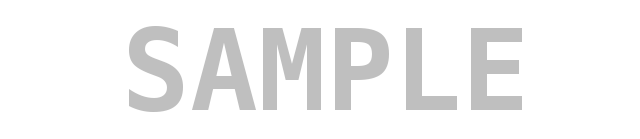
\includegraphics[scale=0.5]{pics/sample.png}
		\caption{Сравнение изображений с разных типов камер} 
		\label{pic:epipol} % название для ссылок внутри кода
	\end{center}
\end{figure}

При этом, как видно по изображению \ref{pic:epipol} (в), сверхшироукольные объективы накладывают на изображение заметные искажения.
Обычно принято рассматривать два вида искажений: тангенциальные и радиальные, но в данном случае тангенциальные принебрежимы по сравнению
 с радиальными и далее рассматриваться не будут. Устранение этих искажений является важной задачей, так как её решение позволяет 
 нивилировать недостатки сверхширокоугольных объективов и применять их для чувствительных к точности передачи формы объектов в кадре задач.

 Одной из таких задач является стереозрение. Несмотря на существование методов, позволяющих оценивать глубину по полным fisheye-снимкам \cite{full_fisheye_stereo}, 
классические методы, требующие ректификации, всё ещё остаются самыми доступными и производительными. Построив систему стереозрения на 
основе ортогонально расположенных сверхширокоугольных камер, можно получить ряд преимуществ перед традиционными камерами, но для этого 
сначала нужно выбрать модель искажений, наиболее точно описывающую данные линзы. [здесь бы сослаться на самого себя, но пока не на что,
и тогда, получается, что принцип этой системы тоже надо бы описать].

Оптическая система была смоделирована в виртуальной среде с применением игрового движка Unity и плагина ZybrVR Dome Tools. %% TODO: что-то ещё про виртуальный опыт 

\subsection{Модели камер "рыбий глаз"}

Сверхширокоугольные линзы изготавливают, закладывая разные виды проекций, их примеры приведены на рисунке \ref{pic:projections}, но 
но реальные линзы не всегда в точности соответствуют им, поэтому для более точного описания принято использовать модели
камер на основе других функций.
Определим основные обозначения. Модель проекции для камеры это функция (обычно обозначаемая $\pi_c(\cdot )$), которая моделирует преобразование 
из точки трёхмерного пространства ($P=[x_c, y_c, z_c]^T$) в поле зрения камеры в точку на плоскости изображения ($p=[u, \nu]^T$). Тогда обратная
проекция - это ... Единичная            % не совсем единичная 
полусфера $S$ с центром в точке $O_c$ описывает поле зрения. На ней также лежит точка $P_C$, являющаяся результатом обратной проекции $\pi^{-1}_c({p})$.
Угол $\theta$ является углом падения для рассматриваемой точки, а угол $\phi$ откладывается между положительным направлением оси $u$ и $O_{i}{p}$. 
% TODO: переписать текст выше более правильным способом
\addimghere{pics/projection_geometry}{0.5}{Схема проекции точки трёхмерного пространства в точку на изображении}{pic:fy_geom}

Основными критериями выбора моделей были: пригодность для моделирования 
сверхширокоугольных линз, простота калибровки и ___популярность___. Существует несколько программных пакетов, позволяющих автоматически калибровать камеры. 
Это kalibr (модели Канналы, Радтан, фов), OdoCamCalib (модели Мея и Канналы), OpenCV (модели Канналы и ) и MATLAB (модель Скарамуззы). Таким образом, далее 
будут рассмотрены основные модели камер, отобранные для сравнения. 

\subsubsection{KB}

Модель Канналы и 
Брандта \cite{opencv_model} реализована в частности OpenCV и описывает радиальные искажения через угол падения луча света на линзу, а не расстояние  
от центра изображения до места падения, как это делалось в более ранних моделях. Авторы посчитали, что для описания типичных искажений достаточно 
пяти членов полинома. Таким образом, указанную модель можно записать следующими уравнениями:

\begin{equation}
\begin{aligned}
	\pi(\mathbf{x}, \mathbf{i}) &=\left[\begin{array}{l}
	f_{x} d(\theta) \\
	f_{y} d(\theta)
	\end{array} \frac{x}{r}\right]+\left[\begin{array}{c}
	c_{x} \\
	c_{y}
	\end{array}\right] \\
	r &=\sqrt{x^{2}+y^{2}} \\
	\theta &=\operatorname{atan} 2(r, z) \\
	d(\theta) &=\theta+k_{1} \theta^{3}+k_{2} \theta^{5}+k_{3} \theta^{7}+k_{4} \theta^{9}
\end{aligned}
\end{equation}

Калибровка камеры по этой модели произведена с помощью библиотеки OdoCamCalib, средня ошибка перепроецирования 
составила 0.012 пикселя. \pdfcomment{mean reprojection error}

\subsubsection{Scaramuzza}

Также большое распространение получила модель Скарамуззы \cite{scaramuzza}, которая легла в основу Matlab Omnidirectional 
Camera Calibration Toolbox, что позволяет быстро и удобно производить калибровку параметров модели.  Она связывает точки 
на изображении с соответствующей им точкой в координатах камеры следующим образом:

\begin{equation}	
    \pi^{-1}(\mathbf{u}, \mathbf{i}) = \lambda \begin{pmatrix}u\\v\\a_0 + a_2 r^2 + a_3 r^3 + a_4 r^4\end{pmatrix},
    %\delta r = k_1\theta + k_2\theta^3 + k_3\theta^5 + k_4\theta^7 + ... + k_n\theta^{n+1}
    \label{eqn:scaramuzza}
\end{equation}
где  $r$ - расстояние от спроектированной точки до центра изображения; $f$ - фокусное расстояние; $\lambda$ - масштабный коэффициент.

Однако для устранения искажений необходима прямая проекция, которая не выражается в явном виде  и находится методом 
Ньютона. \pdfcomment{ проверить точность формулировок }

Средня ошибка перепроецирования составила 0.12 пикселей. %% + ошибка схождения 

\subsubsection{Mei}

Модель Мея \cite{mei} изначально была создана для более эффективного моделирования катадиоптрических камер, но оказалась также весьма
пригодной и для fisheye-камер. 

\begin{equation}
\pi(\mathbf{x}, \mathbf{i})=\left[\begin{array}{l}
	f_{x} \frac{x}{\alpha d+(1-\alpha) z} \\
	f_{y} \frac{y}{\alpha d+(1-\alpha) z}
	\end{array}\right]+\left[\begin{array}{l}
	c_{x} \\
	c_{y}
	\end{array}\right]
\end{equation}

Калибровка камеры по этой модели произведена с помощью библиотеки OdoCamCalib, средня ошибка перепроецирования 
составила 0.013 пикселя.

\subsubsection{Atan}

Эта модель представляет из себя идеальную эквидистантную fisheye-проекцию, которая заложена в использованную виртуальную камеру. 
Она добавлена к сравнению как эталонный способ устранения искажений из предположения, что с ней результаты стереосопоставления будут 
самыми лучшими.  

\begin{equation}
	\pi(\mathbf{x}, \mathbf{i})=\left[\begin{array}{l}
		f_{x} \frac{\theta}{ \sqrt{ \frac{y^2}{x^2} + 1 }} \\
		f_{y} \frac{\theta}{ \sqrt{ \frac{x^2}{y^2} + 1 }}
		\end{array}\right]+\left[\begin{array}{l}
		c_{x} \\
		c_{y}
		\end{array}\right]
	\end{equation}


Таким образом, параметры всех моделей, используемых в сравнении, представлены в таблице \ref{tab:params}.

\pdfcomment{добавить таблицу}

\subsection{Сравнение качества построения карт глубины}

Для сравнения качества построения карты глубины была смоделирована виртуальная стереопара, состоящая из двух камер с объективами 
"рыбий глаз" с полем зрения в $180^\circ$ и принципиальными осями, расположенными под $90^\circ$. При этом объективы камер имеют 
одинаковые параметры, а расстояние между ними составляет 20см. С помощью этой стереопары были получены снимки изображения шахматной доски, 
которые потом были направлены в соответствующие программные пакеты для нахождения параметров каждой модели. Далее с помощью алгоритма [НИР]				% TODO: сделать нормальную ссылку
выполнено устранение искажений в полученных изображениях. По полученной паре изображений можно проводить стереосопоставление. 

\addimghere{pics/sample_simple2cam}{0.7}{Геометрическая модель бинокулярной системы стереозрения}{pic:2cam_scheme}

Здесь область пересечения полей зрения камер $C_0$ и $C_1$ обозначенная красным.
Эта область эквивалентна области пересечения полей зрения двух камер с полями зрения $90^\circ$ (обозначены
оранжевым), повёрнутых на $\beta_0 = \beta_1  = 45^\circ$ в сторону области интереса. Тогда $B$ - база стереопары.
Примеры изображений, полученных в такой конфигурации, приведён на рисунке \ref{pic:dewarped_exmples}. 

\addimghere{pics/4pic_example}{0.7}{Пример исходных изображений с отмеченной областью интереса и снимков виртуальной стереопары}{pic:dewarped_exmples}


Оценка качества построения карты глубины произведена на основе оценки среднеквадратичного отклонения и дисперсии полученных точек 
глубины от их предполагаемой позиции. Виртуальность эксперимента позволяет точно знать положение исследуемого объекта и, соответственно, 
точно определять ошибку. Эффективность стереосопоставления \cite{SGBM} сильно зависит от текстуры наблюдаемого объекта, поэтому для устранения 
её влияния эксперименты были проведены с различными текстурами, а итоговый результат усреднён. Примеры таких текстур приведены на рисунке \ref{pic:textures}. 


\section{Выводы}
\label{conclusion}


\newpage
\bibliographystyle{./config/splncs04}
\bibliography{refs}

\end{document}
